\documentclass[11pt,a4paper,fleqn]{article}
\usepackage{graphicx} 
\usepackage{multirow}
\usepackage{hhline}
\usepackage{amsmath}
\begin{document}
\textbf{CS6140 Machine Learning Fall 2014 Homework 2, Wei Luo }\\
\\
\textbf{PROBLEM 1}\\
\\
 \textbf{B)} Training and testing performance across all four learning algorithms is: \\
 
 \hskip-2cm
 \begin{tabular}{|l|l|l|l|l|}
\hline
 &Decision or &Linear Regression &Linear Regression&LogisticRegression\\
 &Regression Tree&(Normal Equations)&(Gradient Descent)&(Gradeint Descent)\\
\hline
Spambase&Train ACC: 0.91&Train ACC: 0.92&Train ACC: 0.91&Train ACC: 0.92\\
&Test ACC: 0.90&Test ACC: 0.88&Test ACC: 0.90&Test ACC: 0.91\\
\hline
Housing&Train MSE: 26.49&Train MSE: 22.08&Train MSE: 22.13&N/A.\\
 &Test MSE: 24.28&Test MSE: 22.63&Test MSE: 22.58&\\
\hline
\end{tabular}\\
\\ \\
 \textbf{C)} \\
 Confusion Matrix for Decision Tree:\\ \\
\begin{tabular}{cc|c|c|}
\multicolumn{2}{c}{}&\multicolumn{2}{c}{Prediction}\\
\multicolumn{2}{c}{}&\multicolumn{1}{c}{1}&\multicolumn{1}{c}{0}\\
\hhline{~~--}
\multirow{2}{*}{Label}
&1&152&29\\
\hhline{~~--}
&0&14&264\\
\hhline{~~--}
\end{tabular}\\ \\
 Confusion Matrix for Linear Regression:\\ \\
\begin{tabular}{cc|c|c|}
\multicolumn{2}{c}{}&\multicolumn{2}{c}{Prediction}\\
\multicolumn{2}{c}{}&\multicolumn{1}{c}{1}&\multicolumn{1}{c}{0}\\
\hhline{~~--}
\multirow{2}{*}{Label}
&1&162&19\\
\hhline{~~--}
&0&22&256\\
\hhline{~~--}
\end{tabular}\\ \\
 Confusion Matrix for Logistic Regression:\\ \\
\begin{tabular}{cc|c|c|}
\multicolumn{2}{c}{}&\multicolumn{2}{c}{Prediction}\\
\multicolumn{2}{c}{}&\multicolumn{1}{c}{1}&\multicolumn{1}{c}{0}\\
\hhline{~~--}
\multirow{2}{*}{Label}
&1&154&27\\
\hhline{~~--}
&0&10&268\\
\hhline{~~--}
\end{tabular}\\ \\
\newpage \noindent
\textbf{D)} \\
ROC curve for Linear Regression:\\
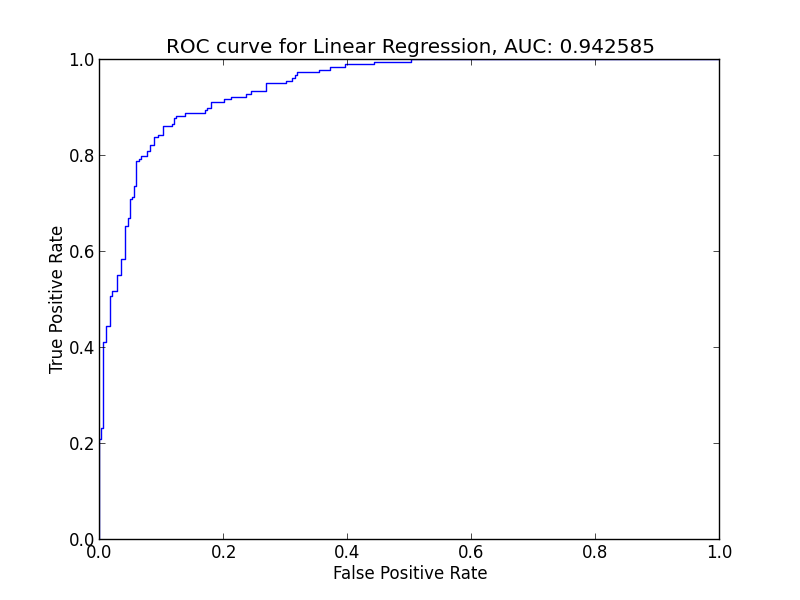
\includegraphics[scale=0.6]{ROC_Linear_Regression.png}\\
ROC curve for Logistic Regression:\\
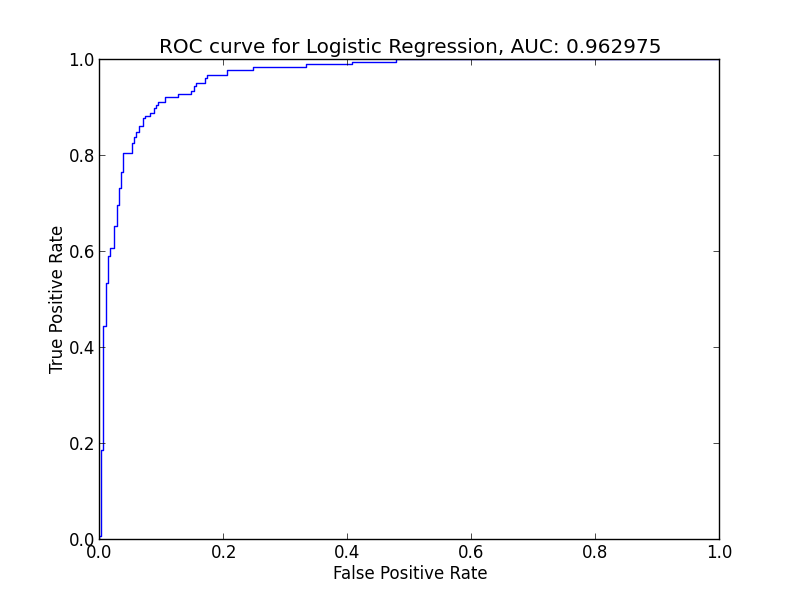
\includegraphics[scale=0.6]{ROC_Logistic_Regression.png}\\
\newpage \noindent
\textbf{PROBLEM 2}\\ \\
Iteration 1, total\_mistake 136\\
Iteration 2, total\_mistake 68\\
Iteration 3, total\_mistake 50\\
Iteration 4, total\_mistake 22\\
Iteration 5, total\_mistake 21\\
Iteration 6, total\_mistake 34\\
Iteration 7, total\_mistake 25\\
Iteration 8, total\_mistake 0\\
Classifier weights:\indent-14.\indent2.52873259\indent5.70717051\indent8.52231457\indent11.32560723\\
Normalized with threshold: \indent0.18062376\indent0.40765504\indent0.60873676\indent0.80897195\\
\\ \\
\textbf{PROBLEM 3}\\ \\
\textbf{b)} 
After training this way, we get a encoder-decoder. With the trained weights, we can encode our data to hidden variables which reduced the size of data. Then the exact data will be kept secret without the weights in our encoder-decoder mechanism. Then, once we need the data, we can decode it with the weights. The weights here are just like keys to encode and decode data.\\
\textbf{c)}
 This encoder-decoder scheme cannot work with one or two hidden variables. Because, the values we get from the sigmoid function is more like binary values. They are distributed near two value. So with $n$ hidden variables, we are more like using $n$ binary values. With that, we can only encode $2^n$ values. So with $N$ input/output values, we need at least $\lceil log_2N \rceil$ hidden variables.\\
\newpage \noindent
\textbf{PROBLEM 4}\\ \\
With our sigmoid function $f(x)$, for a 3-layer neural network, the outputs can be written as
$$g_k(\mathbf{x})=z_k=f(\sum_jw_{kj}f(\sum_iw_{ij}x_i+w_{j0})+w_{k0})$$
The inner $f$ is for hidden variables. If we change it to a linear function, say $lf(x) = ax+b$, then:
\begin{equation}
\begin{aligned}
\nonumber
g_k(\mathbf{x})=z_k&=f(\sum_jw_{kj}lf(\sum_iw_{ij}x_i+w_{j0})+w_{k0})\\
&=f(\sum_jw_{kj}(a_j(\sum_iw_{ij}x_i+w_{j0})+b_j)+w_{k0})\\
&=f(\sum_jw_{kj}(a_j\sum_iw_{ij}x_i+a_jw_{j0}+b_j)+w_{k0})\\
&=f(\sum_jw_{kj}a_j\sum_iw_{ij}x_i+\sum_jw_{kj}(a_jw_{j0}+b_j)+w_{k0})\\
&=f(\sum_i(\sum_jw_{kj}a_jw_{ij})x_i+\sum_jw_{kj}(a_jw_{j0}+b_j)+w_{k0})\\
\end{aligned}
\end{equation}
Let $w'_{ki}=\sum_jw_{kj}a_jw_{ij}$, $w'_{k0}=\sum_jw_{kj}(a_jw_{j0}+b_j)+w_{k0}$, we have
$$g_k(\mathbf{x}) = f(\sum_iw'_{ki}x_i+w'_{k0})$$
Which is equivalent to a two-layer network output.\\
Therefore, a three-layer network with linear hidden units can be reshaped to a two-layer network.\\
With a two-layer network, we cannot solve non-linearly separable problem XOR because: Say, we have weights $w_1\ w_2\ w_3$, basis $b$, and a threshold $t$ for the network. For the XOR problem, we need:\\
\begin{tabular}{cc}
(1) $w_0b+w_10+w_21 \ge t$&(2) $w_0b+w_11+w_20 \ge t$\\
(3) $w_0b+w_10+w_20 < t$&(4) $w_0b+w_11+w_21 < t$\\
\end{tabular}\\
From (1)(2), we have $2w_0+w_1+w_2 \ge 2t$, from (3)(4), we have $2w_0+w_1+w_2 < 2t$ which is a contradiction due to the XOR problem itself is not linearly separable. We can not solve this problem with such network. Similary for other non-linearly separable problems since the function is linear.\\
\newpage \noindent
\textbf{PROBLEM 5}\\ \\
\end{document}